\section{Projekt Narra}
\par Narra je projekt s volně dostupným zdrojovým kódem, který se zabývá anotací a~propojením audiovizuálních médií a~textu. Podobně jako YouTube má také veřejně dostupné API po dokončení bude soužit umělcům, filmařům a~dalším, kteří chtějí vytvářet otevřený příběh (open narrative), nebo editovat videa. Dokumentaristé mohou tento projekt využít pro rozsáhlejší díla, díky nabídnutému relevantnímu obsahu s metadaty. Projekt zastřešuje FAMU CAS, které poskytuje práci pro více jak 30 studentů dokončujících Bakalářské a~Magisterské studium.
\par S první myšlenkou projektu Narra přišel v roce 2002 - 2003 Eric Rosenzveig a~Willy LeMaitre spolu s dalšími mediálními umělci a~programátory. Dílo bylo rozdělené na tři části. První "plaListNetWork" byl opensource software vyvinutý na základě konzultací s umělci o audiovizuálním obsahu a~rozhraním pro vizualizaci. Umožňoval práci více uživatelů na různých místech a~pomocí textových poznámek upravovat popisky skladeb a~videí. Druhý "disPlayList" bylo veřejně přístupné rozhraní pro streamování medií z~playListNetWork. Jednalo se o webovou aplikaci, která vizualizovala výsledná videa do grafu, ze kterého šel pomocí klíčových slov tvořit další celek. "Ressemblage", neboli poslední část byl výsledkem práce umělců používajících novou technologii práce s médii.
\par V projekt Open Narrative se zapříčinil nejvíce umělec Eric Rosenzveig a~redaktor Tomáš Dobruška na FAMU v letech 2010 - 2015. Díky penězům z~grantu mohou pokračovat ve vývoji spolu s KSI FIT ČVUT.

\section{Technologie v projektu Narra} 
\par Narra je psaná v jazyce Ruby a~poskytuje REST-API pro komunikaci se světem. Další použité technologie jsou Sidekiq, OmniAuth, MongoDB a~Rails. Všechny tyto komponenty zajišťují stabilní jádro aplikace, na které je možné připisovat další balíčky (gem), jako v případě mé bakalářské práce. Pro začátek jsem se musel seznámit s doménovým modelem celé aplikace.

\begin{figure}[H]
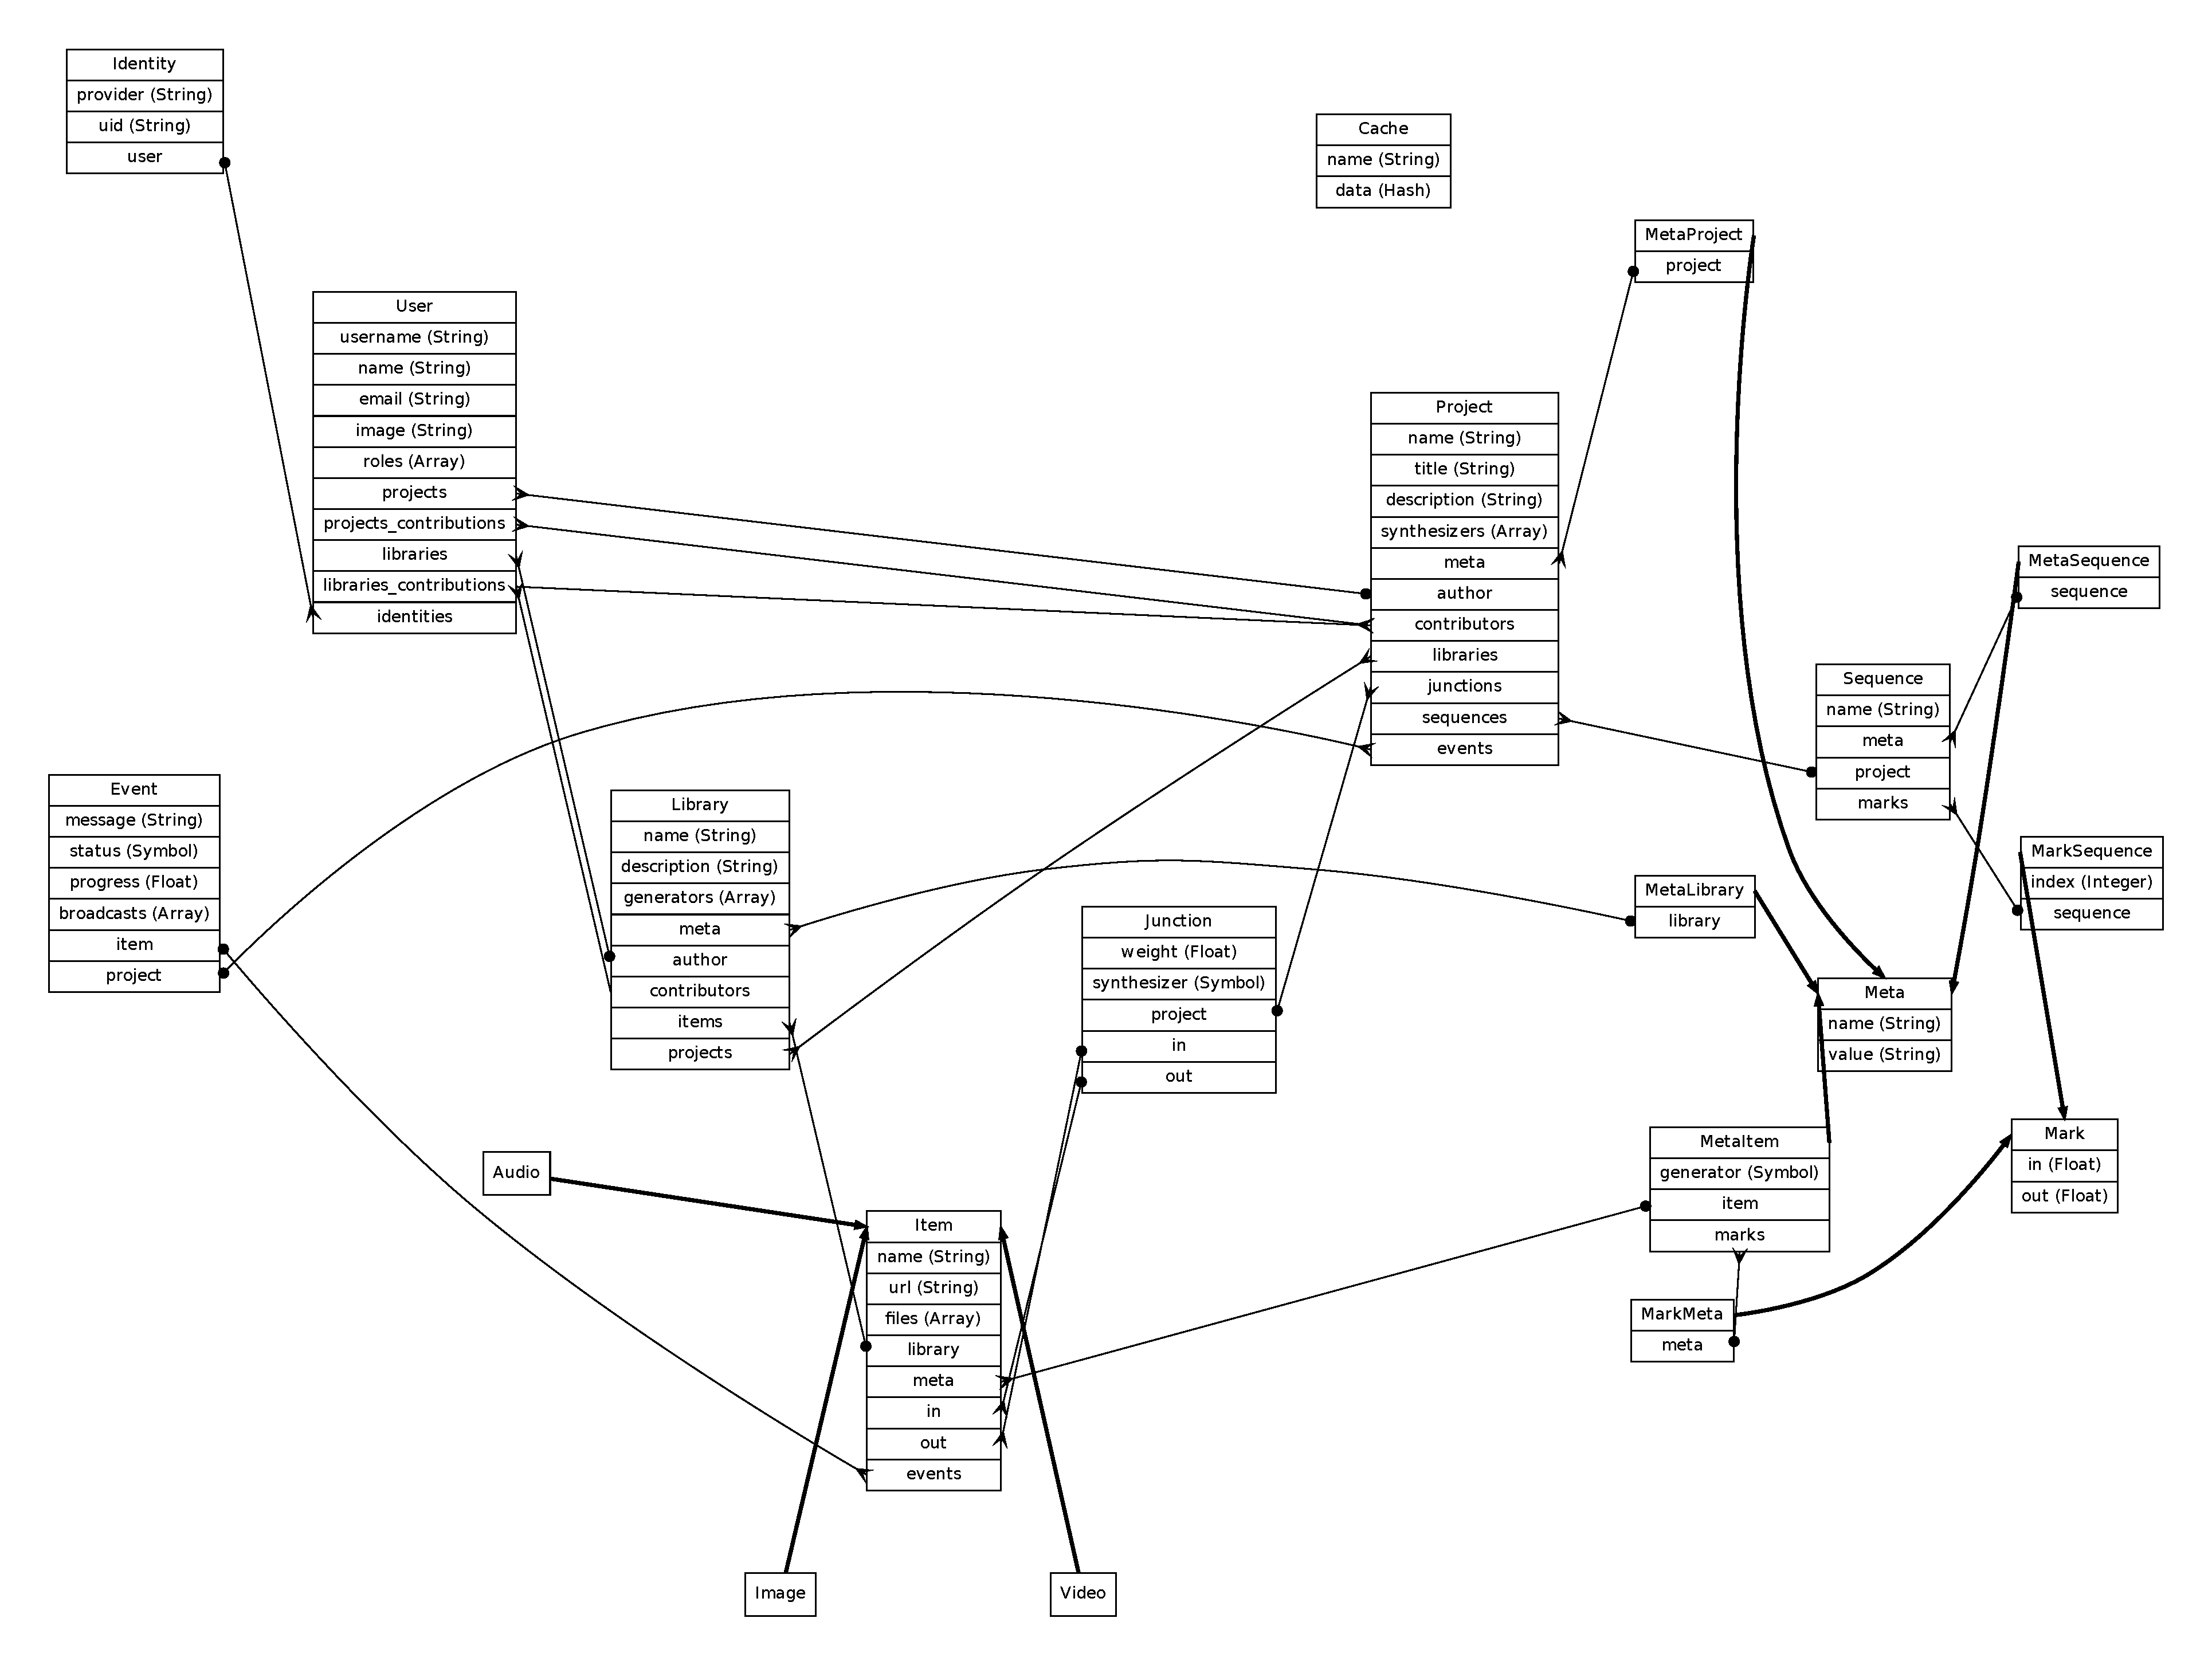
\includegraphics[width=1\textwidth]{./obrazova_priloha/domain_full.pdf}
\caption{Doménový model celého projektu Narra}
\end{figure}

\par User reprezentuje přihlášeného uživatele, který chce používat aplikaci. Každý uživatel má vazbu na projekt a knihovnu. Entita Item je reprezentována jménem souboru, url videa a vlastními staženými soubory. Dále obsahuje vazby na knihovnu ve které jsou uložena videa. Další vazba je na entitu MetaItem, která reprezentuje generátor pro metadata. MetaItem je statická třída, která obsahuje vazbu na Meta. Meta už obsahuje příslušné jméno a položky platné pro popis metadaty.

\begin{figure}[H]
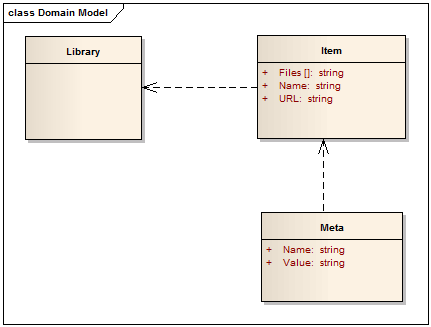
\includegraphics[width=1\textwidth]{./obrazova_priloha/domain_my.png}
\caption{Doménový model mé části Narry}
\end{figure}
\par Moje část aplikace je tvořena entitami Item, Meta a Library. Entita library reprezentuje celou knihovnu videí, se kterou se bude lokálně pracovat. Item je jeden konkrétní prvek u kterého je potřeba provést validaci a inicializaci pomocí url. Jméno pro konkrétní prvek je reprezentováno stringem a url je také string. Pro jednoduché volání budu mít vytvořenou třídu Connector, která bude provádět inicializace, validaci, popis metadaty a stažení videa a případných titulků.